\section{Identification with the Koenigs function}
\label{a:sec:koenigs}

Some time after the search of \cref{a:sec:GA} had been abandoned, a dynamical
argument emerged that explains why no elementary closed form should be expected.
In short: $A(p)$ is a value of the Koenigs linearising function of the logistic
map, and that function is known to be non-elementary throughout the parameter
range required. This section makes the identification precise; the next supplies
the obstruction.

\subsection{Koenigs linearisation}
\label{a:sec:koenigsdef}

\begin{definition}[Koenigs function]
\label{a:def:koenigs}
Let $f_r(z) = rz(1-z)$ have a fixed point at $z=0$ with multiplier
$r=f_r'(0)$ satisfying $0<|r|<1$. Koenigs \cite{Koenigs1884} proved that there is
a unique function $\psi_r$, holomorphic in a neighbourhood of the origin,
satisfying the Schr\"oder equation
\begin{equation}
\label{a:eq:schroder}
\psi_r\bigl(f_r(z)\bigr) = r\,\psi_r(z),
\qquad
\psi_r(0)=0,
\qquad
\psi_r'(0)=1 .
\end{equation}
Equivalently,
\begin{equation}
\label{a:eq:koenigslimit}
\psi_r(z) = \lim_{n\to\infty}r^{-n}f_r^{\circ n}(z)
\end{equation}
uniformly near the origin. The normalisation $\psi_r'(0)=1$ is equivalent to
$\psi_r(z)/z\to1$ as $z\to0$.
\end{definition}

\noindent
The Koenigs function is a change of coordinate that straightens the dynamics: in
the $\psi_r$ coordinate the nonlinear map $f_r$ becomes multiplication by $r$
(\cref{a:fig:koenigs}). Standard accounts are Milnor \cite{Milnor2006} and
Carleson and Gamelin \cite{Carleson1993}. Throughout this chapter
$f_r(z)=rz(1-z)$ is exactly \cref{a:eq:logistic}, with $z=w_n$ and
$f_r(z)=w_{n+1}$, and the multiplier is $r=2p\in(0,1)$ --- an attracting fixed
point, which is the classical Koenigs setting.

\begin{figure}[ht]
\centering
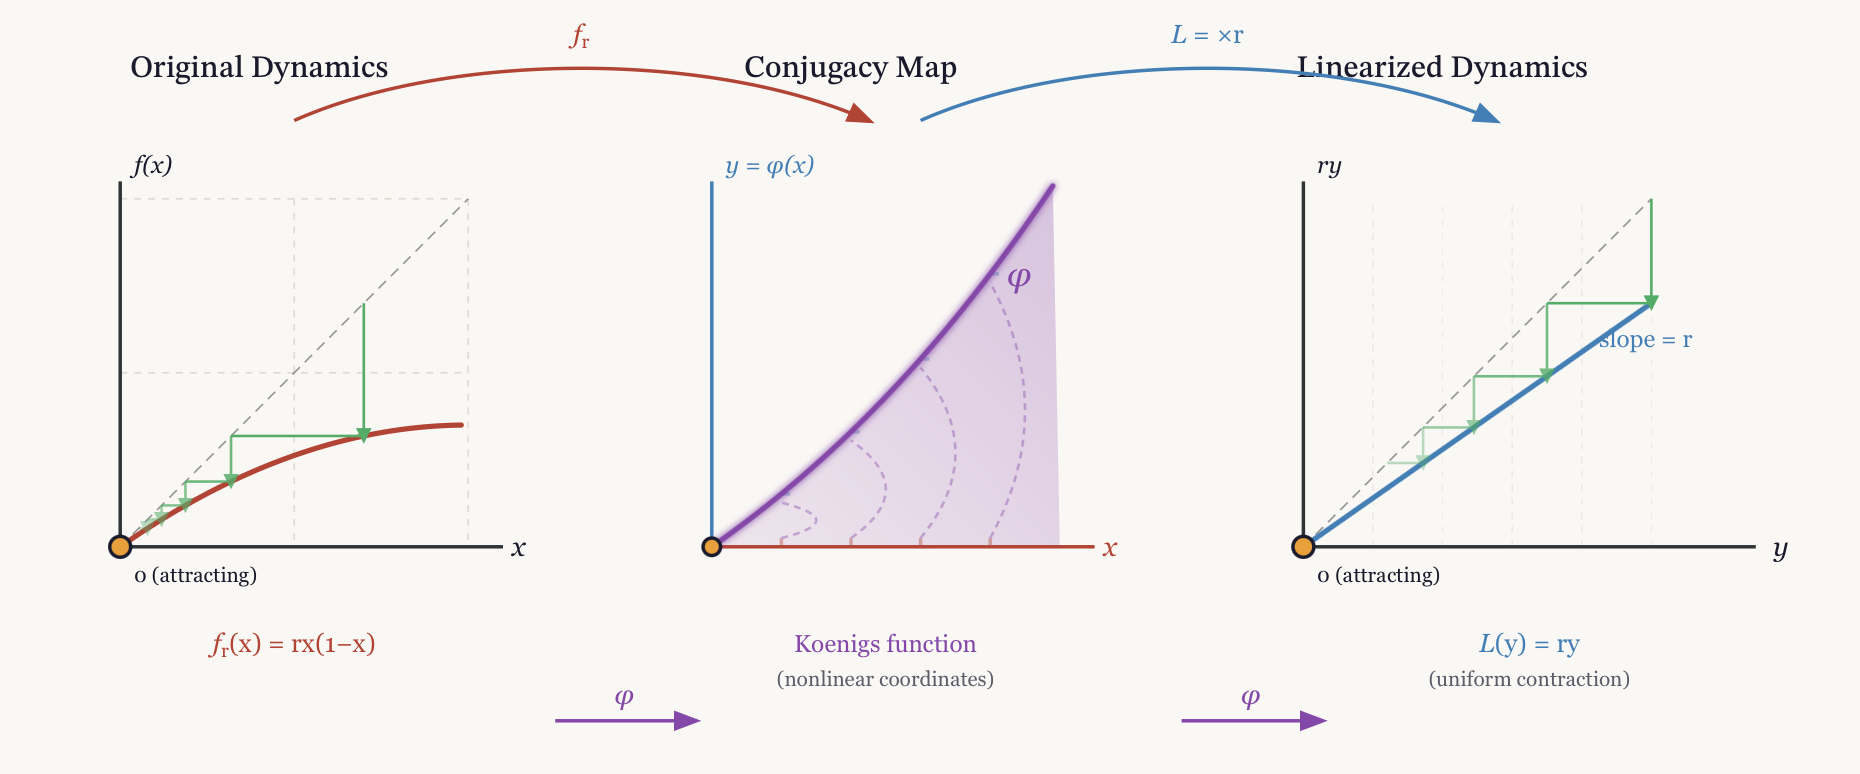
\includegraphics[width=0.72\textwidth]{figures/figure2_koenigs_linearization.png}
\caption{Koenigs linearisation of the logistic map near an attracting fixed point.
The nonlinear dynamics $x\mapsto f_r(x)=rx(1-x)$ are conjugated by $\psi_r$ to the
linear map $y\mapsto ry$; the diagram displays the functional relation
$\psi_r(f_r(x)) = r\psi_r(x)$ and the role of $\psi_r$ as the coordinate change
that straightens the dynamics.}
\label{a:fig:koenigs}
\end{figure}

\subsection{The identity \texorpdfstring{$A(p)=2\psi_r(\tfrac12)$}{A(p) = 2 psi(1/2)}}
\label{a:sec:identity}

The local Koenigs function is initially defined only in a neighbourhood of $0$.
For $r\in(0,1)$ the origin is attracting on the real line and the interval $(0,1)$
lies in its real basin: starting from $w_0=\tfrac12$, one has $w_n\to0$. On that
basin the limit
\begin{equation}
\label{a:eq:basinkoenigs}
\Psi_r(w_0) := \lim_{n\to\infty}r^{-n}f_r^{\circ n}(w_0)
\end{equation}
exists and agrees with the local conjugacy near $0$, since the normalisation
$\psi_r'(0)=1$ gives $\psi_r(w_n)/r^n\sim w_n/r^n$ along the orbit.

\begin{proposition}
\label{a:prop:AisKoenigs}
For $p\in(0,\tfrac12)$ and $r=2p$,
\begin{equation}
\label{a:eq:AeqKoenigs}
A(p) = 2\,\Psi_r\!\lrb{\tfrac12}
= 2\lim_{n\to\infty}r^{-n}f_r^{\circ n}\!\lrb{\tfrac12} .
\end{equation}
\end{proposition}

\begin{proof}
Along the orbit, whenever $w_n$ lies in the local domain, iterating
\cref{a:eq:schroder} gives $\psi_r(w_1)=r\psi_r(w_0)$, hence
$\psi_r(w_0)=\psi_r(w_1)/r$, and by induction
\begin{equation}
\label{a:eq:induction}
\psi_r(w_0) = \frac{\psi_r(w_n)}{r^n}\qquad\text{for every }n .
\end{equation}
Passing to the limit, $\psi_r(w_0) = \lim_n\psi_r(w_n)/r^n$. Since $w_n\to0$ and
$\psi_r(z)/z\to1$ as $z\to0$, replacing $\psi_r(w_n)$ by $w_n$ in the limit is
legitimate, and $\psi_r(w_0)=\lim_n w_n/r^n$. Comparing with \cref{a:eq:Aw} and
using $w_n = S_n/2$ and $w_0=S_0/2=\tfrac12$ gives
$A(p) = 2\Psi_r(\tfrac12)$.
\end{proof}

\noindent
We write $A(p)=2\psi_r(\tfrac12)$ as a shorthand for this basin value of the
Koenigs conjugacy, not as a naive evaluation of a power series beyond its
guaranteed disc of convergence; the relation between the germ and the basin is
taken up in \cref{a:rem:basin}. Thus every question about an elementary closed
form for $A(p)$ is tied to the nature of that conjugacy at multiplier $r=2p$.

\subsection{Conjugacy with the quadratic family}
\label{a:sec:quadratic}

The logistic family is affinely conjugate to the canonical quadratic family, and
the correspondence is used repeatedly below.

\begin{lemma}
\label{a:lem:affine}
The logistic map $f_r(x)=rx(1-x)$ is affinely conjugate to $P_c(z)=z^2+c$ with
\begin{equation}
\label{a:eq:cofr}
c = c(r) := \frac{2r-r^2}{4} .
\end{equation}
Under this correspondence the interval $r\in(0,1)$ maps to $c\in(0,\tfrac14)$.
\end{lemma}

\begin{proof}
Seek $h(x)=ax+b$ with $h\circ f_r\circ h^{-1} = P_c$. The substitution
$x = -z/r+\tfrac12$ (for $r\neq0$) yields a monic quadratic; matching coefficients
gives $c=(2r-r^2)/4$. Since $c(r)$ increases on $(0,1)$, with $c(0)=0$ and
$c(1)=\tfrac14$, the image of the branching window is $(0,\tfrac14)$.
\end{proof}

\begin{figure}[ht]
\centering
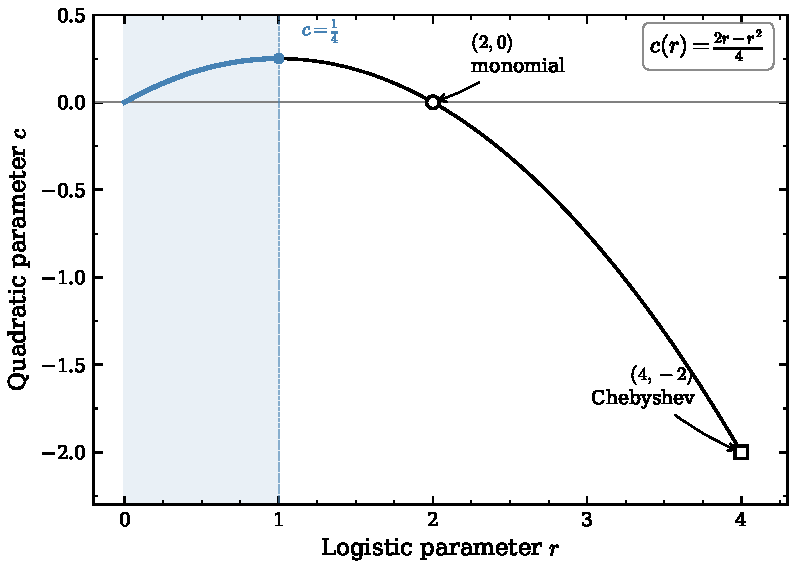
\includegraphics[width=0.66\textwidth]{figures/figure1_parameter_conjugacy.pdf}
\caption{The affine parameter correspondence $c(r) = (2r-r^2)/4$ between the
logistic family $f_r(x)=rx(1-x)$ and the quadratic family $P_c(z)=z^2+c$. The
shaded segment is $r\in(0,1)$, the subcritical branching window, which maps to
$c\in(0,\tfrac14)$. The two integrable parameters, $r=2$ ($c=0$, monomial) and
$r=4$ ($c=-2$, Chebyshev), lie outside it; see \cref{a:app:integrable}.}
\label{a:fig:conjugacy}
\end{figure}

The interval $c\in(0,\tfrac14)$ is the real diameter of the main cardioid of the
Mandelbrot set: a fixed point of $z^2+c$ with multiplier $r$ has coordinate
$z_\ast=r/2$, and its fixed-point equation gives
$c = z_\ast-z_\ast^2 = r/2-r^2/4$, with the endpoint $r\uparrow1$ approaching the
parabolic cusp $c=\tfrac14$, which is criticality. This locates the parameter
range geometrically; its role in the obstruction argument is fixed in the next
section, and it is not used as evidence for any closed-form claim.
